\documentclass[a4paper, 12pt]{article}
\usepackage[utf8]{inputenc}
\usepackage[left=2cm, right=2cm, top=2cm, bottom=2cm]{geometry}
\usepackage[colorlinks=true, citecolor=blue, linkcolor=black, urlcolor=blue]{hyperref}
\usepackage{graphicx} %allow use \includegraphics
\usepackage{amsthm}
\usepackage{mathtools}
% \usepackage{natbib}

\usepackage[round,authoryear,sort]{natbib}
% show dois as links on references
\usepackage{doi}
% Remove extra space between references
\usepackage{references/natbibspacing}
% Use a different font

\usepackage[section]{placeins}
\usepackage{tabularx}
\usepackage{makecell}
\usepackage{multirow}
\usepackage{enumitem}
\usepackage[english, brazil]{babel}
\usepackage{changepage}
\usepackage{comment}
\usepackage[doublespacing]{setspace}
\usepackage{placeins}
\usepackage{capt-of}
\usepackage{caption}
\usepackage{rotating}
\usepackage[table,xcdraw]{xcolor}
\usepackage{siunitx}

\usepackage{booktabs}
\usepackage{titlesec}
\titleformat{\section}{\normalfont\Large\bfseries}{\Roman{part}-\thesection}{1em}{}
\titleformat{\subsection}{\normalfont\bfseries}{\Roman{part}-\thesubsection}{1em}{}
\titleformat{\subsubsection}{\normalfont\itshape}{\Roman{part}-\thesubsubsection}{1em}{}

\usepackage{float}

\usepackage{pdfpages}
\usepackage{lastpage}
\usepackage{fancyhdr}
\usepackage{titletoc}


\titlecontents{section}
  [0pt] % Espaço esquerdo
  {} % Espaço acima
  {} % Formato do título (neste caso, vazio)
  {} % Espaço entre o título e o número da página
  {} % Formato do número da página
  [\vspace{1ex}] % Espaço após cada entrada

\begin{document}

\begin{titlepage}
   \begin{center}
        \vspace*{0.5cm}
        % \newgeometry{left=2.5cm, right=1.5cm,}
        \small{\textbf{UNIVERSIDADE DE SÃO PAULO\\INSTITUTO DE ASTRONOMIA, GEOFÍSICA E CIÊNCIAS ATMOSFÉRICAS\\PROGRAMA DE PÓS GRADUAÇÃO EM GEOFÍSICA}}
        
        \vfill
        \large{Research Title:\\\textbf{Micropaleomagnetism}}
            
        \vfill
        \normalsize{
            \textbf{Third Semester Report}\\
            \textbf{Period:} 04/23 - 10/23
            \vfill
     
       %\includegraphics[width=0.4\textwidth]{university}
        \begin{center}
        \begin{tabular}{l l}
            \textbf{PhD Candidate:} & Gelson Ferreira de Souza Junior\\
            \textbf{Supervisor:}  & Leonardo Uieda\\
            \textbf{Co-supervisor:} &  Ricardo Ivan Ferreira da Trindade\\
        \end{tabular}
        \end{center}

        
            % \textbf{PhD Candidate:} Gelson Ferreira de Souza Junior\\
            % \textbf{Supervisor:} Leonardo Uieda\\
            % \textbf{Co-supervisor:} Ricardo Ivan Ferreira da Trindade\\
            %\textbf{Linha de pesquisa:} Modelagem numérica, Tectonofísica, Margens convergentes e Margens rifteadas
        }
        
        \vfill
        \normalsize{São Paulo, October 2023}
            
   \end{center}
\end{titlepage}
% \restoregeometry
%Custom abstract
\singlespacing
\selectlanguage{english}
\section*{\centering{\footnotesize{ABSTRACT}}}
    \begin{adjustwidth}{18pt}{38pt}
            \setstretch{1.0}{
            \footnotesize
            % Paleomagnetic data are usually obtained from whole cylindric samples, where the signal results from the sum of magnetic moments from hundreds of thousands to millions of magnetic particles within the sample volume. 
            % This usually includes both stable and unstable remanence carriers.
            % Recently, magnetic microscopy techniques allowed the investigation of individual grains by directly imaging their magnetic field. 
            % However, the determination of the magnetic moments of individual grains is hindered by the intrinsic ambiguity in the inversion of potential field data, as well as by the large number of grains found in any one microscopy image. In our previous work,
            % we presented a fast, semi-automated algorithm capable of estimating the position and magnetization of each ferromagnetic (l.s) source using only the magnetic microscopy data. 
            % Our algorithm works in three steps: (i) we first apply image processing techniques to identify and isolate data window boundaries for each source; (ii) with these window boundaries, the position of the sources is estimated using Euler deconvolution; and finally (iii) using the  position information, the algorithm is able to estimate the magnetic dipole moment direction and intensity for each source through an overdetermined linear inverse problem using a dipolar approximation. 
            % The method does not require any type of additional information about the sample or the sources. Tests with simple synthetic data show the high effectiveness of the methodology for recovering the position and magnetic information for both dipolar and non-dipolar sources. 
            % More complex synthetic data including over 100 different magnetic particles were devised to emulate real rock data. 
            % Results obtained on these data also show the feasibility and robustness of the algorithm to semi-automatically estimate the position and magnetic moment of a large number of particles. 
            % This is further confirmed through an application to real data in which we are able to retrieve the expected bimodal isothermal remanent directions that were induced in the sample. 
            % Given its semi-automatic nature, its low processing cost, and the possibility of simultaneous inversion of the magnetic moment of a great number of magnetic particles, the methodology here proposed is a step forward in enabling paleomagnetic applications of magnetic microscopy.

        In the context of paleomagnetism, we face the challenge of obtaining crucial information about magnetic sources present in rock samples using non-invasive techniques without the need for costly and limiting additional methods. In our previous work, we proposed an innovative approach aimed at obtaining a priori information about magnetic sources based solely on data generated by magnetic microscopy. Our approach begins with the identification of the region where the signal from magnetic particles is present in the rock sample. Using an edge detection algorithm, we isolate these areas of interest, creating "slices" of data. We then apply the Euler deconvolution (ED) technique to these data windows to estimate the three-dimensional position of the magnetic particles, assuming they behave as point dipolar sources. The results of our synthetic tests demonstrate the effectiveness of our methodology. We tested point dipolar sources with varying magnetization in terms of direction, intensity, and depth. The algorithm not only identified all the source windows, including the weakest ones, but also produced minimal differences between the modeled position and the position estimated by ED. Furthermore, we conducted tests with complex magnetization sources and the Euler algorithm continued to work effectively even for non-dipolar fields. The magnetic moment recovery was also very effective for dipolar and non-dipolar synthetic sources, which enabled further tests with real data samples (speleothems). In the latter, the magnetic directions estimated were also coherent with the induce isothermal remanent magnetization. However, some limitations with our approach were detected and this report mainly represents an attempt to tackle and solve these limitations, and also strategies to improve the proposed methodology.
            
            
        }
        \end{adjustwidth}


% \newpage
% \selectlanguage{brazil}
% \section*{\centering{\footnotesize{RESUMO}}}
% 	\begin{adjustwidth}{18pt}{38pt}
% 	    \setstretch{1.0}{
%      \footnotesize
%      Os dados paleomagnéticos são geralmente obtidos a partir de amostras cilíndricas completas, onde o sinal resulta da soma dos momentos magnéticos de centenas de milhares a milhões de partículas magnéticas dentro do volume da amostra. Isso normalmente inclui portadores de remanescência estáveis e instáveis. Recentemente, as técnicas de microscopia magnética permitiram a investigação de grãos individuais através da imagem direta de seus campos magnéticos. No entanto, a determinação dos momentos magnéticos de grãos individuais é dificultada pela ambiguidade intrínseca na inversão dos dados do campo potencial, bem como pelo grande número de grãos encontrados em qualquer imagem de microscopia. Apresentamos um algoritmo rápido e semi-automatizado capaz de estimar a posição e a magnetização de cada fonte ferromagnética (l.s) usando apenas os dados de microscopia magnética. Nosso algoritmo funciona em três etapas: (i) aplicamos técnicas de processamento de imagem para identificar e isolar as fronteiras das janelas de dados para cada fonte; (ii) com essas fronteiras de janelas, a posição das fontes é estimada usando a deconvolução de Euler; e, finalmente, (iii) usando as informações de posição, o algoritmo é capaz de estimar a direção e intensidade do momento dipolar magnético para cada fonte através de um problema inverso linear sobredeterminado usando uma aproximação dipolar. O método não requer nenhum tipo de informação adicional sobre a amostra ou as fontes. Foram realizados testes de sensibilidade para estimar a estabilidade de nossa rotina em relação à profundidade das partículas, razão sinal-ruído e não dipolaridade das fontes. Testes com dados sintéticos simples mostram a alta efetividade da metodologia na recuperação das informações de posição e magnetismo tanto para fontes dipolares quanto não dipolares. Dados sintéticos mais complexos, incluindo mais de 100 partículas magnéticas diferentes, foram criados para emular dados reais de rochas. Os resultados obtidos com esses dados também demonstram a viabilidade e robustez do algoritmo para estimar semi-automaticamente a posição e o momento magnético de um grande número de partículas. Isso é confirmado por meio de uma aplicação a dados reais em que conseguimos recuperar as direções esperadas de remanescência isotérmica bimodal que foram induzidas na amostra. Dada a sua natureza semi-automática, baixo custo de processamento e possibilidade de inversão simultânea do momento magnético de um grande número de partículas magnéticas, a metodologia aqui proposta representa um avanço na capacidade de aplicar a microscopia magnética em estudos paleomagnéticos.
%         }
% 	 \end{adjustwidth}
\selectlanguage{english}
\doublespacing
\newpage

\listoffigures

\listoftables
\newpage

\tableofcontents
\newpage

    
%\part{Research groundwork}\label{content}
% This section of the monograph is devoted to describing the foundational aspects of the research, which led to the submission of a scientific paper to Geophysics, Geochemistry, and Geosystems.

\section{Introduction}


\begin{figure}[tb!]
  \centering
  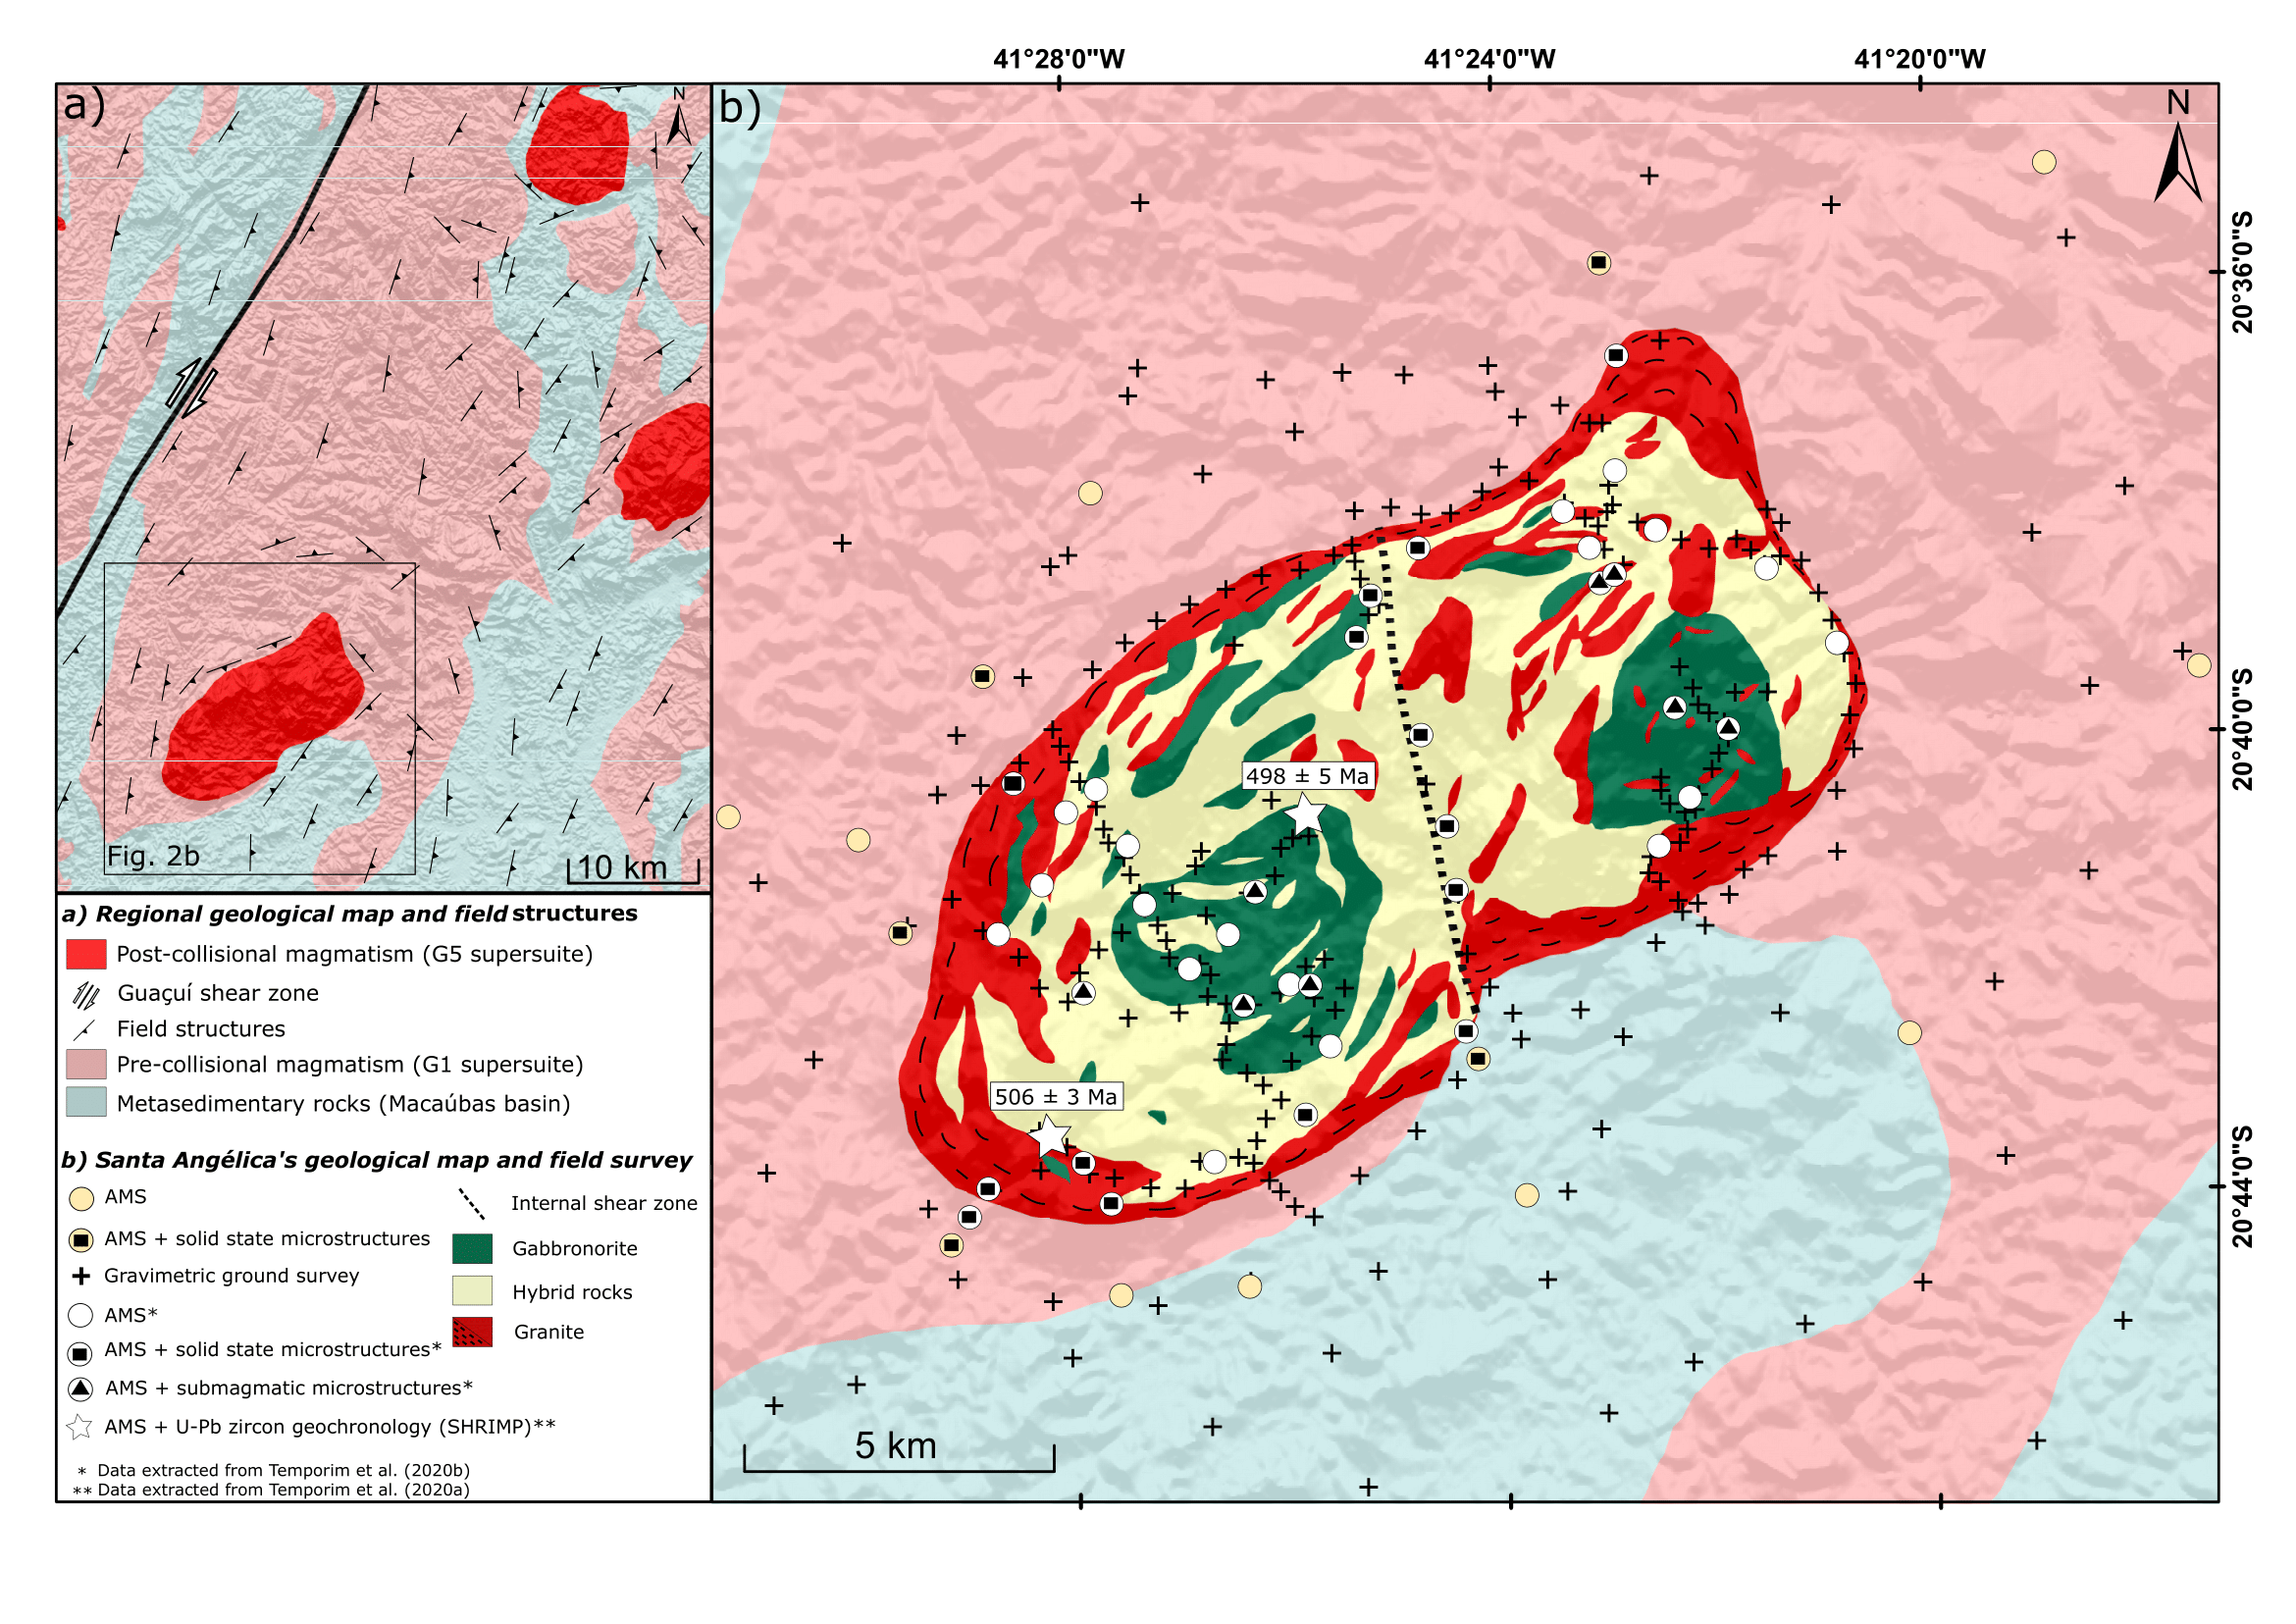
\includegraphics[width=1\linewidth]{figures/geology.png}
  \caption{
    % Addressing computational challenges in magnetic microscopy with extensive datasets.
    % a) Complete synthetic dataset featuring all N observation points including areas lacking relevant information.
    % b) Streamlining data through pre-selected windows reduces the dataset size for inversion, ensuring efficiency without compromising final results.
      }
  \label{euler1}
\end{figure}

\section{Methodology}

The open dataset for this study involves the collection of 227 gravity stations (Figure~\ref{geology}b). The Gravity measurements were obtained using a Lacoste and Romberg gravimeter (model G, ±0.01 mGal), while orthometric altitude was determined using a Differential Global Positioning System (DGPS) device (± 0.3 m). Data on gravity were collected at varying intervals: 

\begin{enumerate}[label=(\roman*)]
    \item detailed: with one station approximately every 0.3 km, forming three profiles intersecting the SAIC (Figure~\ref{geology}b), two traversing each lobe, and one along the internal shear zone.
    \item regional: in the country rocks, the data coverage was approximately one station per 4 km, aiming to complement the existing regional gravity dataset.
\end{enumerate}


The Bouguer anomaly was obtained and interpreted by \citet{Souza-Junior2021}. However, in this study, we will calculate the gravity field at the same point on the reference ellipsoid, thus obtaining the Bouguer disturbance. To accomplish this, a few processing stages were necessary, as it is described below.

\subsection{Altitude Transformation}\label{altitude}

The initial step involved converting orthometric altitudes ($H$) from both the gravimetric dataset in this study and the topographic database (with a spatial resolution of 30 m $\times$ 30 m, Figure~\ref{heights}a). To achieve this, we obtained the mesh containing the geoid level ($N$) for the study area (with an approximated spatial resolution of 10 km $\times$ 10 km, Figure~\ref{heights}b). The orthometric topography and geoid height databases were acquired from pyGMT database \citep{gmt} and plotted with the aid of the PyGMT library \citep{pygmt}. The geoid height grid underwent an interpolation process to generate a mesh with the same resolution as the orthometric topography, which was possible using the Verde python library \citep{verde2018}. Subsequently, the geometric altitude ($h$) was calculated by adding both meshes ($h = H + N$,~Figure~\ref{heights}c).

\begin{figure}[H]
  \centering
  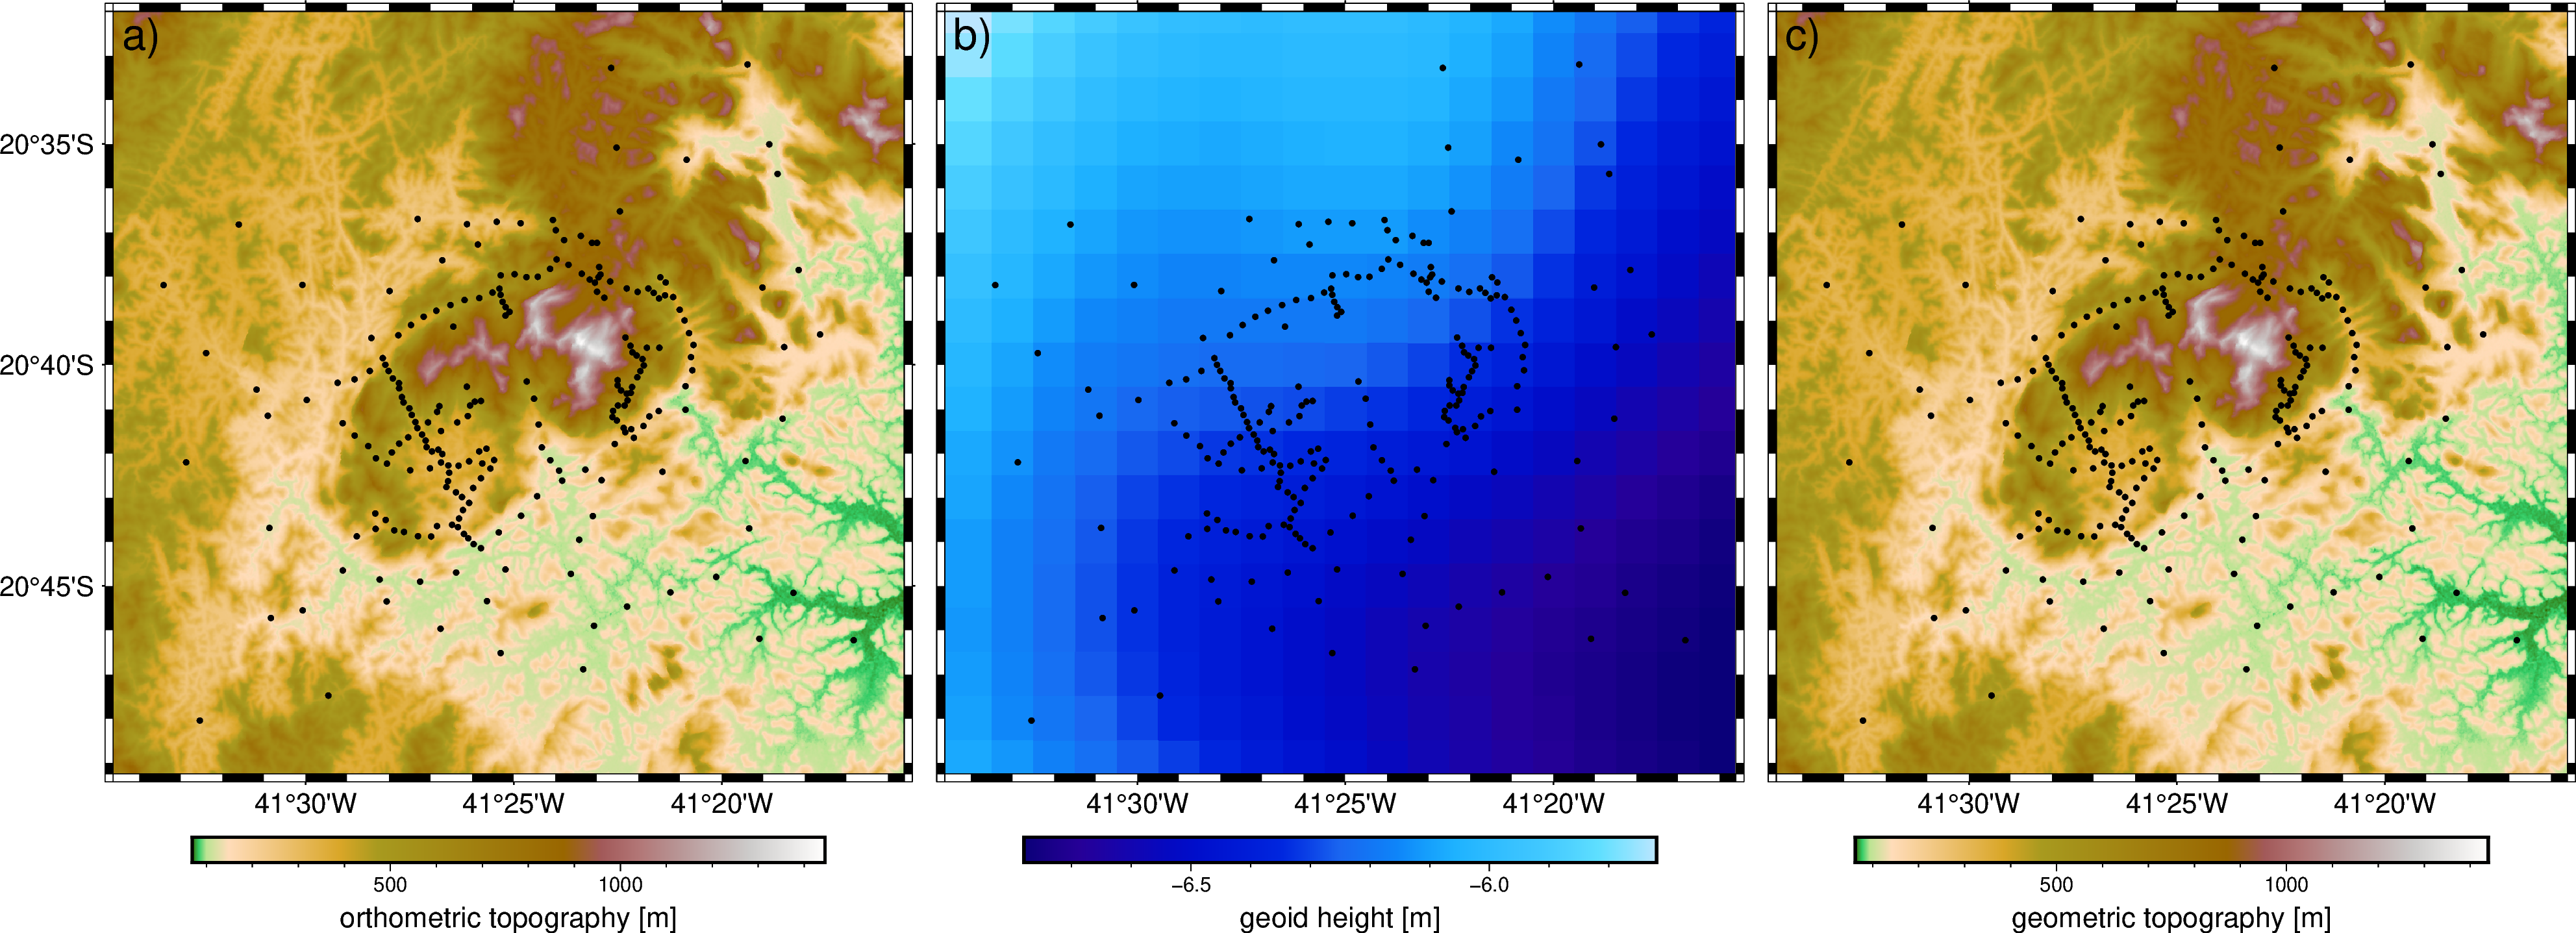
\includegraphics[width=1\linewidth]{figures/heights.png}
  \caption{
    Topographic grids of the study area. a) Orthometric topography. b) Geoid height. c) Geometric topography. 
      }
  \label{heights}
\end{figure}


\subsection{Normal Gravity}
An anomaly is usually a term related to the difference between a measured data (\textit{e.g.}, $g_{\text{obs}}$) and the theoretical or expected data in that specific point \citep{Encyclopedia_solid_earth_geophysics}. The calculation of the theoretical gravity is obtained with a model of a rotational bi-axial ellipsoid \citep{Pasteka2017}. This called ``normal Earth'' has a few characteristics: 

\begin{enumerate}[label=(\roman*)]
    \item The same mass (M) and center of mass as the Earth;
    \item The same angular velocity as the Earth; and
    \item The potential on its surface is equal to the potential of the geoid.
\end{enumerate}
The magnitude of the gradient of the gravity potential generated by the normal Earth ellipsoid, which includes the gravitational and centrifugal effects, is called normal gravity $(\gamma)$. The calculation of this normal gravity was performed using the World Geodetic System 1984 (WGS 84) by the Boule package \citep{Boule2020}, which implements the closed-form formula of \citet{Li2001} and calculate the $\gamma$ given the latitudes and the geometric heights. This is the reason why the first step consists of the conversion of the orthometric to geometric heights. 

\subsection{Topographic Correction}

Once the normal gravity is ``corrected'', a further correction must be performed to remove the effects of the rocks between the ellipsoid and the observation point, since the effect of the topography is not predicted in the theoretical gravity \citep{Encyclopedia_solid_earth_geophysics}. This called ``Bouguer correction'' ($\delta g_{B}$) usually is computed by an infinite slab of rock that fills the space between the geoid level and the measured point \citep{Lowrie1997}, \textit{i.e.}, the slab has the orthometric height ($H$). The Bouguer correction formula is given by:

\begin{equation}
{
\delta g_{B} = 2 \pi G \rho H},
\end{equation}

\noindent{where $G$ is the universal gravitational constant ($6.67428\times10^{-11}~m^3 kg^{-1} s^{-2}$) and and $\rho$ is the density of the Bouguer infinite-slab, which, by standard, generally assumes the crust's average density of $2670~kg~ m^{-3}$ \citep{Hinze2003}.}

However, this presumption of an infinite-slab can lead to errors in areas with very pronounced topographic variations and/or when the choice of plate density is made incorrectly \citep{Chapin1996}. Figure~\ref{heights} shows that the study area has topographic variations greater than 1000 meters, which will most likely cause unwanted calculation errors. Thus, it is possible to apply a method of topographic correction \citep[\textit{e.g.,}][]{Nagy2000} based on the topography mesh (Section~\ref{altitude}), since our goal is to determine the gravity disturbance we will use the geometric heights. In this sense, each grid cell of the digital elevation model was converted into a flat prism of 30 m $\times$ 30 m $\times$ $h$ m, this creates a volumetric model for the geometric topography. Subsequently, the gravity effect of each regular prism with a constant density ($\rho = 2670~kg~m^{-3}$) can be computed, which gives the topography's gravity effect ($g_T$).

\subsection{Bouguer Disturbance}
Depending on the chosen reference gravity model, two distinct types of anomaly variations might be considered: gravity anomalies and gravity disturbances. The geodetic gravity anomaly is defined as the distinction between gravity on the geoid and normal gravity on the reference ellipsoid \citep{Blakely1996}. Conversely, the gravity disturbance is defined as the difference in the fields at the same point on the reference ellipsoid. According to \citet{Encyclopedia_solid_earth_geophysics} the gravity disturbances are more suitable for geophysical purposes. When applying the normal gravity and terrain corrections, the Bouguer disturbance ($\delta g_{b}$) can be determined by:

\begin{equation}
{
\delta g_{b} = g_{obs} - \gamma - g_T}.
\end{equation}

\subsection{Residual-Regional Separation}

The Bouguer anomaly, or Bouguer disturbance in this case (Figure~\ref{gravity}a), is said to be the result from the density contrast between rocks \citep{Amelio1997}. However, potential fields are additives and usually consist of two components: one with large-wavelength and other with short-wavelength. Anomalies of large wavelength are caused by the effects of deeper density contrasts and are referred to as regional anomalies \citep{Telford1990}. On the other hand, short-wavelength anomalies, known as residual anomalies, are induced by anomalous mass distribution in the shallow crust and are employed for their study \citep{Lowrie1997}. Therefore, studying more restricted area requires the application of a regional-residual separation technique to isolate the effect of the targeted bodies. 

In our study, we applied a first-degree polynomial fit onto the Bouguer disturbance map (Figure~\ref{gravity}a) to predict the regional component of the regional/deeper sources using Verde python package \citep{verde2018}, as shown in Figure~\ref{gravity}b. Then, this regional trend was subtracted from the Bouguer disturbance to generate the residual anomalies map (Figure~\ref{gravity}c).
These anomalies, or residuals, are attributed to localized and shallow subsurface bodies.

\begin{figure}[H]
  \centering
  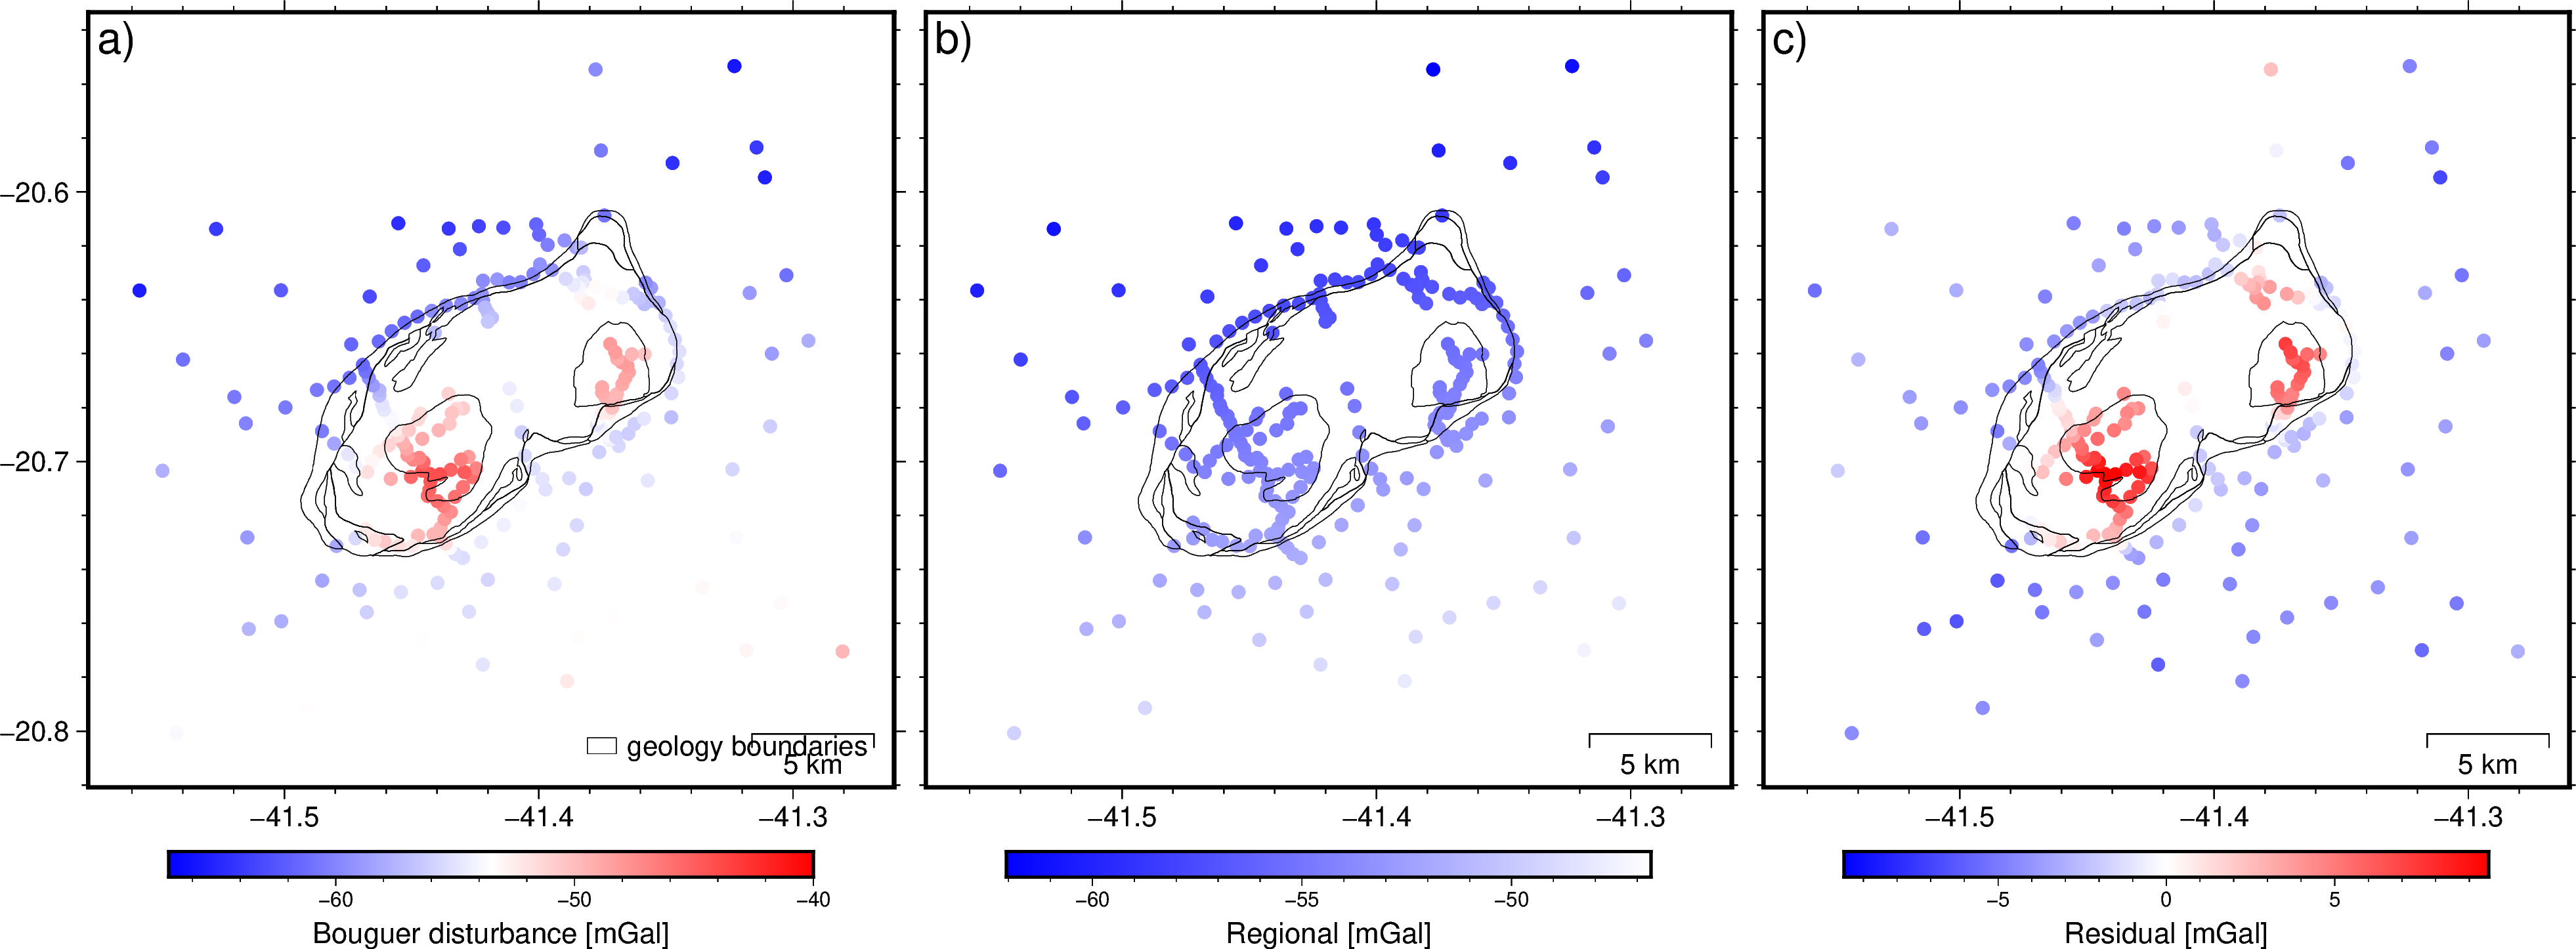
\includegraphics[width=1\linewidth]{figures/gravity.png}
  \caption{
    SAIC's gravimetric maps. a) Bouguer disturbance. b) Regional anomaly obtained with the first-degree polynomial fit of the Bouguer disturbance. c) Residual Bouguer disturbance.
      }
  \label{gravity}
\end{figure}


\subsection{Data Interpolation with Equivalent Layer}

Potential field surveys often are datasets of irregular measurements from flight lines or along the terrain's surface. The processing usually involves interpolating onto a regular grid at a constant height for further visualization and processing (\textit{e.g.,} reduction-to-the-pole, upward continuation and derivatives calculations) \citep{Soler2021}. An effective method for performing this task is through equivalent sources \citep{Dampney1969}, also known as an equivalent layer. This technique involves defining a finite set of geometric bodies (e.g., point sources) beneath observation points and adjusting their coefficients to replicate the measured field. The technique can be used to predict the values for the gravimetric and magnetic field at any point, such as regular grids and different heights, while also outperforming others 2D interpolators like the minimum curvature or bi-harmonic splines \citep{Soler2020, Uieda2020}.

\subsubsection{Derivatives and Gradients}

With the same equivalent layer it is possible do determine derivatives by disturbing the regular grid with a value $\Delta \alpha$, $\alpha = x, y, z$, and predicting the residual Bouguer disturbance at that point, following the finite-difference method:

\begin{equation}
    {\frac{\partial f}{\partial x} = \frac{f(x + \Delta x, y, z) - f(x - \Delta x, y, z)}{2\Delta x}},
\end{equation}

\noindent{likewise for the other derivatives. Afterwards, they can be applied on the formulas:

\begin{align}
    HG &= \sqrt{\left (\frac{\partial f}{\partial x}\right )^2+\left (\frac{\partial f}{\partial y} \right )^2}~~~~~~~~~\text{and} \\
    TG &= \sqrt{\left (\frac{\partial f}{\partial x}\right )^2+\left (\frac{\partial f}{\partial y} \right )^2+\left (\frac{\partial f}{\partial z} \right )^2},
\end{align}

\noindent{so it is possible to calculate the horizontal gradient \citep[HG,][]{Cordell1985} and the total gradient \citep[TG,][]{Roest1992Magnetic}.}

\section{Application to synthetic data}

\section{Discussion}

\subsection{Prior information and uniqueness of solutions}

Working with potential field data might be very tricky once there is too much ambiguity involved during data modeling, thus to obtain unique and reliable results from data inversion it is necessary to provide as much prior information as possible.
One way to circumvent the ambiguity is to incorporate prior information about the subsurface structure, such as the positioning of a known source of magnetization.
Magnetic field measurements are more sensitive to changes in magnetization near the source that is causing the anomaly.
When the position of the source is known, it constrains the model to be as consistent as possible with the observed data, hence increasing the likelihood of obtaining unique solutions.
\citet{Oliveira2015Estimation} proved that the magnetization directions (Dec and Inc) recovered by the least squares estimator are sensitive to great variations in the horizontal coordinates of the center of the magnetic sources, but are practically insensitive to variations in depth.
Thus, they consider the ED method as an adequate technique to estimate the central positions that will be used as prior information for inversion.
This occurs mainly because, when well performed, the recovery of the source's horizontal coordinates is considerably accurate, while the vertical coordinate can undergo greater variation even though it still provides satisfactory results \citep{Silva20033D, Melo2013}.
This remark is also better observed in our simple synthetic sample where the estimated horizontal positions slightly deviate from the true values, which implies small misfit values in the recovered magnetic directions.
Although the estimated magnetic moment for the said sample is satisfactory, this magnetic parameter is more affected by the variations in the depth of the source, which is probably caused by ambiguities.
In summary, in order to estimate all magnetic parameters as precisely as possible the ED must be executed within a data window containing the lowest amount possible of noise since that high-frequency noise sensibility is one of the ED's main limitations.

\subsection{A critical examination of the source detection}

Since the pioneering work of \cite{Egli2000}, many methodologies were proposed for solving the inverse problem o micromagnetic data, and for the purpose of comparison we separate them into two categories based on the main estimated parameter by the inversion procedure.
In the first type of approach, the main goal is usually to estimate average magnetization by inverting the whole sample superficial magnetization data commonly by means of unidirectional problem, uniform directions with non-negative variable dipole moments \citep[e.g.,][]{Weiss2007}, including performance enhancement in the spatial domain \citep[e.g.,][]{Myre2019} or frequency domain  \citep[e.g.,][]{Lima2013}.
This methodology can be used to remarkably estimate the average magnetic direction and the total moment direction with the assumption that the particles were all magnetized in the direction of the same induced field \citep[sIRM and/or NRM in basalts,][]{Weiss2007}.
However, this assumption is not always true when dealing with complex samples (i.e., more than one stable direction), which leads to the same drawbacks as the classic paleomagnetic measurements using bulk samples.
The second type of approach has the goal of finding the individual source magnetic properties, which can be done by either inverting the dipole moment of a single source within a cropped section of an upward continued anomaly map \citep[e.g.,][]{Lima2016, Fu2020} or by the insertion of additional information of the sources’ shape, such as micro-computed tomography (microCT) \citep[e.g.,][]{Fabian2019, DeGroot2018, DeGroot2021}.
The latter further allows unique estimation of magnetic moment configuration of even higher orders components through spherical harmonics expansion constrained by micromagnetic models \citep[e.g.,][]{CortesOrtuno2021, CortesOrtuno2022}.
Such outstanding techniques come with some troubles of having to mechanically select the data for inversion or dealing with the weaknesses of the additional method used.
The MicroCT, for example, is a popular non-destructive technique for high-resolution imaging of the material internal structures, and yet, it is accompanied by some limitations when it comes to paleomagnetic studies: firstly, the technique has a spatial resolution on the order of micrometers, which is not sufficient to directly image the fined grained single-domain magnetite \citep{DeGroot2018}.
The microCT also struggles to discern ferromagnetic (\textit{l.s.}) from non-magnetic/antiferromagnetic minerals, as pointed out by \cite{DeGroot2021}, since they usually have similar densities and therefore similar X-ray attenuation \citep{Cnudde2013}.
In any case, the major limitation of microCT lies in the trade-off between the resolution and the sample size, requiring small sample volumes to achieve higher resolutions causing the technique to be too time-consuming.

Our proposed methodology has the goal of finding each individual source’s dipole moment components without the trouble of mechanically selecting cropped data or needing any type of additional information.
However, to better examine its advantages and disadvantages we first need to point out the strengths and weaknesses of the technique used in the detection of sources, the Laplacian of Gaussian (LoG) kernel \citep{Marr1980}.
The LoG is a computer imaging technique that is able to identify regions where the intensity changes abruptly by convolving the image with the LoG filter, and is the result of the combination of the Gaussian blur and Laplacian filter \citep{gonzalez2018}.
The Laplacian filter is able to highlight the regions where the intensity changes rapidly.
On the other hand, the Gaussian blur is a smoothing filter for high-frequency noise, which reduces the likelihood to generate artifacts.
Hence, the result of this LoG operation can identify blobs as regions above a certain threshold, this threshold crossing determines what are brighter spots (local maxima) surrounded by a darker background.
It is also scale-invariant by detecting blobs of different sizes and intensities, a feature achieved by varying the sizes of the Gaussian filter.
The advantages of the methodology are (i) high-accuracy blob detection; (ii) scale-invariant for images with different intensities/sizes of objects; while also being (iii) robust to the presence of noise due to the Gaussian smoothing filter.
While the main drawbacks of the LoG blob algorithms are: (i) being computationally expensive/time-consuming when dealing with larger images and (ii) the requirement of parameter adjustments, such as the threshold and the kernel sizes.

The total gradient anomaly (TGA) might be considered the ideal image to be used as input for the LoG blob detection algorithm for potential field studies (micro and/or macroscale).
The TGA highlights the subsurface sources by generating a map of positive magnetic anomalies concentrated within their edges.
This technique is widely used in aeromagnetic surveys to determine the boundaries of sources by calculating the magnetic gradient in all Cartesian directions and displaying those regions where the gradient has maximum values, which is a local maxima distribution.
Hence. The application for micromagnetic measurements comes with all the advantages and drawbacks previously mentioned because is highly dependent on the selection of a good data window.
Nonetheless, the windows generated isolate the main magnetic signal’s region of each source.
This guarantees that our thresholding approach (see section~\ref{dipole-reliability}), for both ED and dipolar inversion, is performed using the critical slice of the micromagnetic data, giving satisfactory parameters approximation and fast results as shown in the synthetic data.

The complex synthetic data allows better observation of the strengths and limitations of the windows approach.
The main strengths that can be mentioned are: (i) the applied technique not only detects most of the modeled sources but also (ii) most of the recovered magnetic parameters have considerably low errors, especially in the directions, usually less than 5° (Figure~\ref{complex-synthetic-comparison}a).
(iii) The magnetic moments obtained from well-individualized sources tend to not deviate much from the real values (Figure~\ref{complex-synthetic-comparison}b) when $R^2$ and SNR scores are considered high ($\geq 0.85$ and $\geq 5$, respectively) (Figure~\ref{complex-synthetic-comparison}c-d).
(iv) Shallow particles grouped in clusters are usually well individualized during window selection, as well as (v) some isolated particles that produce a weak magnetic signal.
The major limitations observed were: (i) the blob detection fails when there are sources too close, grouping them into the same window, thus causing an erroneous result both for Euler deconvolution and for the magnetic parameters.
(ii) The very same occurs when there is a source under another, in this case, the magnetic signal is the sum of both.
(iii) In clusters of larger and/or deeper particles, although the method individualizes them well, the magnetic signal of the neighboring particles can considerably influence the result of the inversion, especially the estimated dipole moment (cluster in the Figure~\ref{complex-synthetic-comparison}b with the highest misfit values).
As expected, there is a direct relationship between the dipole intensity and depth with the observed errors.
It is clear from the error bars in Figure~\ref{complex-synthetic-comparison} that deep-seated sources and/or particles with small dipole moments generate worse results, essentially because they will produce weaker anomalous fields in the magnetic maps.
Note nonetheless, that even sources with small dipole moments when close to the surface are adequately modeled by our method, because of the trade-off between signal and noise for grains near the sensor.


\subsection{Reliability of dipole moment approximation}
\label{dipole-reliability}

Our approach relies in the premise of assuming the magnetic anomaly within
the data window is a response of a dipolar source.
The latter is true when working
with particle signals in the SD magnetic domain state since they are uniform magnetized particles with strong dipolar anomalies.
However, \cite{Nagy2017} reported that particles within the PSD domain can record the paleomagnetic field for longer (than SD ones) periods of time, being the stabler and also with strongly non-dipolar characteristics.
Therefore the application of the proposed algorithm to natural samples should fail for those PSD particles.
\cite{CortesOrtuno2022} give important insights about the matter, they showed that PSD state particles present more accurate inversion results when considering the non-dipole components for small sample-sensor distances (\textless 1 $\mu$m), but for larger sensor distances the dipole as approximations are remarkably accurate, as the higher-order moments decay rapidly with distance and therefore have less
influence on the particle's magnetic signal.
Thus, our approach can be considered reasonable to work with both particle SD and PSD states signals.
The latter happens mainly due to the sensor height being usually greater than 5 $\mu m$, considering a particle on the immediate surface of the sample the higher-order moments are already quite attenuated, thus circumventing the prominent problems described for non-dipolar components. This is corroborated by our non-dipolar synthetic sample showing the almost complete attenuation of non-dipolar components at distances greater than 5 $\mu m$.

Despite the excellent signal-to-noise ratio that the SMM provided with the
proximity of the sensor to the sample, it is worth mentioning that the
measurement noise can still overshadow the responses of very weak/small, or
deep particles, generating unreliable inversion results.
Therefore, it is necessary to keep a check to determine if the inversion reached a satisfactory prediction, such as the coefficient of determination and the
signal-to-noise ratio suggested by \citep{CortesOrtuno2021}.

While the windows approach violates the fundamental theory of the inversion problem that  requires the sampled area to be finite and encapsulated by the inversion domain to ensure the uniqueness of results \citep{Baratchart2013,Lima2013}, our technique is similar to the  one reported by \cite{Weiss2007}.
The last-mentioned involves thresholding the long-distance interaction
of each dipole in the SMM data, which excludes the effect of other dipoles by setting their contribution to zero, resulting in a sparse matrix that permits faster calculations.
In contrast to this approach, we employ the TGA map to select the windows and isolate the area containing the main signal of the desired dipole, while the area out of the boundaries of the window is less sensitive to variation in magnetic parameters of this particular source, hence we exclude them from the inversion domain.
This technique allows us to obtain the 3D positioning and an approximation of the dipole moment components of hundreds of sources within a few seconds, while the inversion is fast the time bottleneck of our methodology is associated with the blob detection process.
\section{Final Remarks}
The obtained results align seamlessly with the geological characteristics of the SAIC. The presence of positive peaks directly corresponds to the mafic cores, while positive values observed over the mixture zone and negative values along the granitic borders further reinforce the consistency of the applied technique. These findings not only validate the efficacy of the equivalent layer methodology employed but also the interpolated residual product does not show the typical edge effect associated with 2D interpolation. The success of this gravity processing approach underscores its potential as a reliable tool for investigating the SAIC's (and other intrusive bodies) subsurface structures in future gravimetric modeling.

\newpage
\section*{Data and Code Availability}

The Python source code used to produce all results and figures presented here is available at \url{https://github.com/Souza-junior/Disciplina_Verao_IAG_2024} under the MIT open-source license. The SAIC's gravimetric ground survey data are available at \url{https://doi.org/10.6084/m9.figshare.25215725} under the CC-0 license.


We used all open-source packages in the Jupyter Notebook programming environment \citep{Kluyver2016}. We performed coordinates manipulations, generated regular grids, and data interpolation with the aid of Verde \citep{verde2018}. Boule package \citep{Boule2020} for calculation of the normal gravity. Harmonica package \citep{harmonica2020} was used in the terrain gravity effects correction and also for the equivalent layer technique. The orthometric and geoid models were acquired from the GMT database \citep{gmt} and the map generation was handled by the PyGMT package \citep{pygmt}.


\newpage
\singlespacing
\bibliographystyle{references/apalike-doi}
\bibliography{references/cas-refs}

\newpage


% \section*{}

% \vfill  % Espaço vertical automático
% \thispagestyle{empty}  % Remove cabeçalho e rodapé desta página

% \begin{center}
% \begin{tabular}{c}
%   \toprule
%   \newline \\
%   \Huge\bfseries\fontsize{20}{20}\selectfont{LATINMAG EXTENDED ABSTRACT} \\
%   \newline \\
%   \bottomrule
% \end{tabular}
% \end{center}

% \vfill  % Espaço vertical automático
% \newpage  % Pula para uma nova página
% \includepdf[pages=-]{PDF/GEOMGF_GFSJ_1.pdf}


% %%%%%%%%%%%%%
% \newpage
% \section*{}
% \vfill  % Espaço vertical automático
% \thispagestyle{empty}  % Remove cabeçalho e rodapé desta página

% \begin{center}
% \begin{tabular}{c}
%   \toprule
%   \newline \\
%   \Huge\bfseries\fontsize{20}{20}\selectfont{EGU ABSTRACT} \\
%   \newline \\
%   \bottomrule
% \end{tabular}
% \end{center}

% \vfill  % Espaço vertical automático
% \newpage  % Pula para uma nova página

% \includepdf[pages=-]{PDF/EGU23-4479-print.pdf}

% 
\end{document}
